

\subsection{The Challenges: Foregrounds and Systematics}
\label{sec:foregrounds_systematics}

\vspace{-0.05in}

The search for primordial $B$ modes poses the most stringent requirements on foreground removal 
and control of systematic effects. A tentative target for the CMB Probe is to constrain the tensor-to-scalar ratio with an 
uncertainty that is a factor of 50-100 smaller than the current upper limit $r < 0.07\, (95\%),$ that is, to reach 
$\sigma(r)\lesssim0.0005$ 
limited by foreground uncertainties. 
%in the presence of foregrounds and accounting for systematic effects. 
%According to data from \planck\ and sub-orbital experiments,
Foregrounds already dominate the signal. The large reduction in the size of 
the final error will require exquisite measurements and modeling of their properties. 

To ascertain that the uncertainty on the measurement is dominated by statistics, or foreground 
uncertainties, rather than systematic errors, the contribution due to instrumental systematic effects 
should be $\sigma(r)\lesssim0.0001.$ To achieve these unprecedented levels 
the mission design, execution, and data analysis will be driven by control of systematic uncertainties. 
\begin{figure}[ht!]
\vspace{-0.15in}
\hspace{-0.2in}
\begin{center}
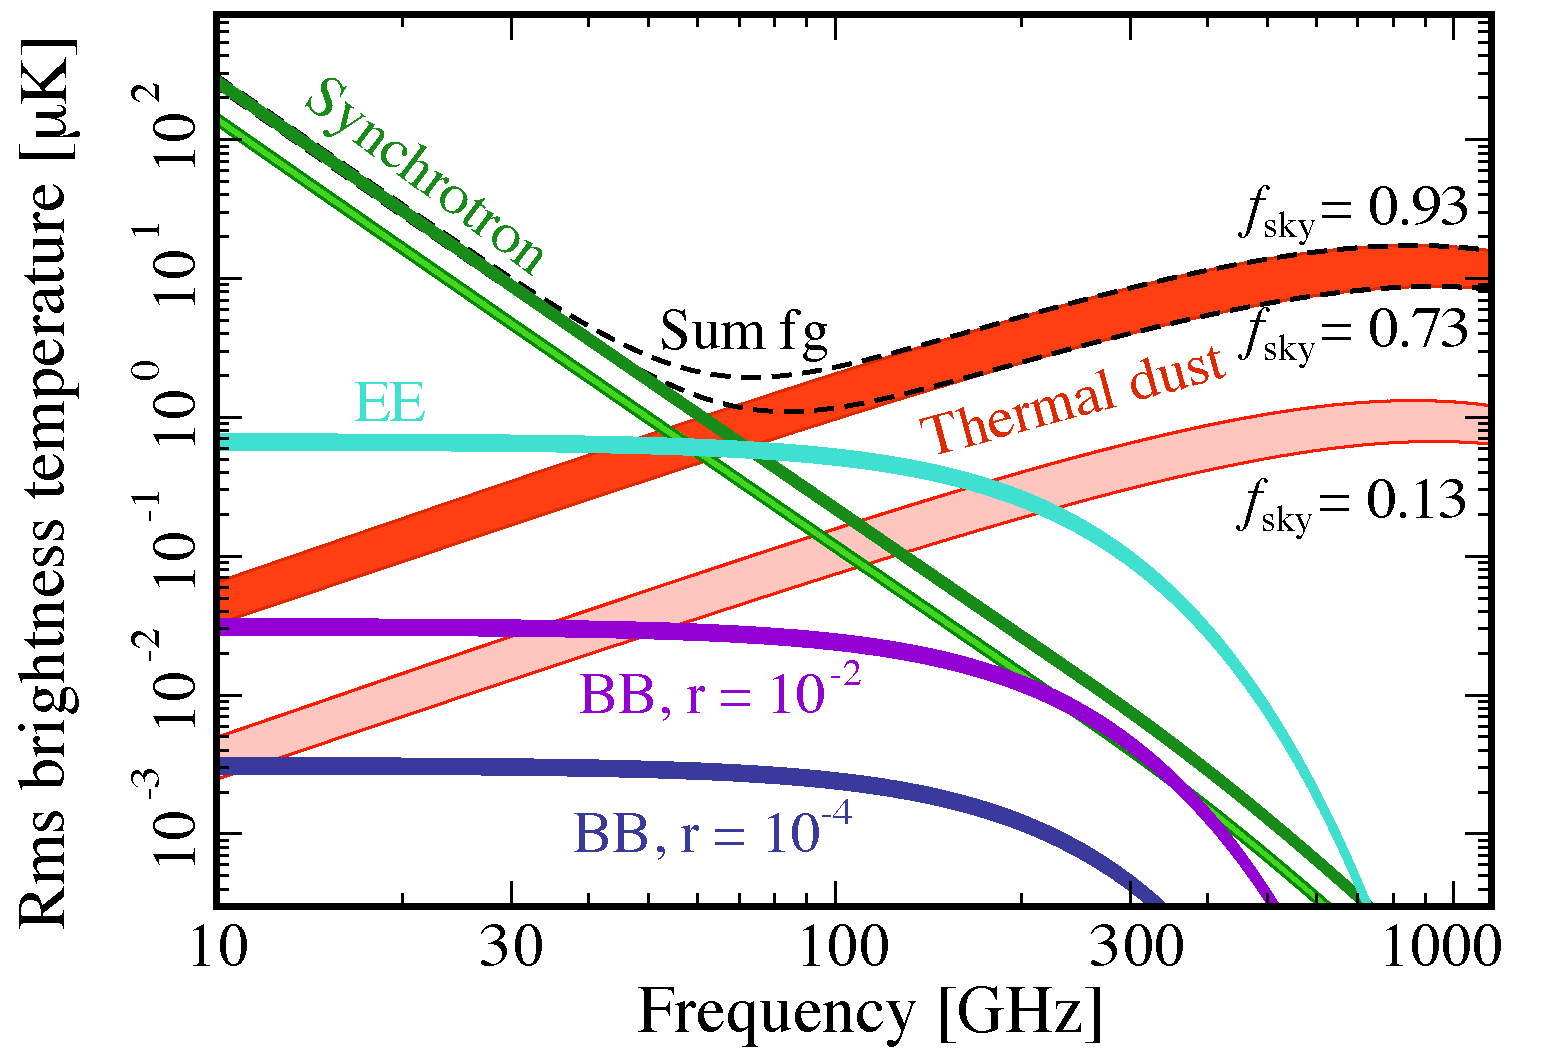
\includegraphics[width=3.2in]{Figures/overview_pol_v4_fsky_noplanck.pdf}
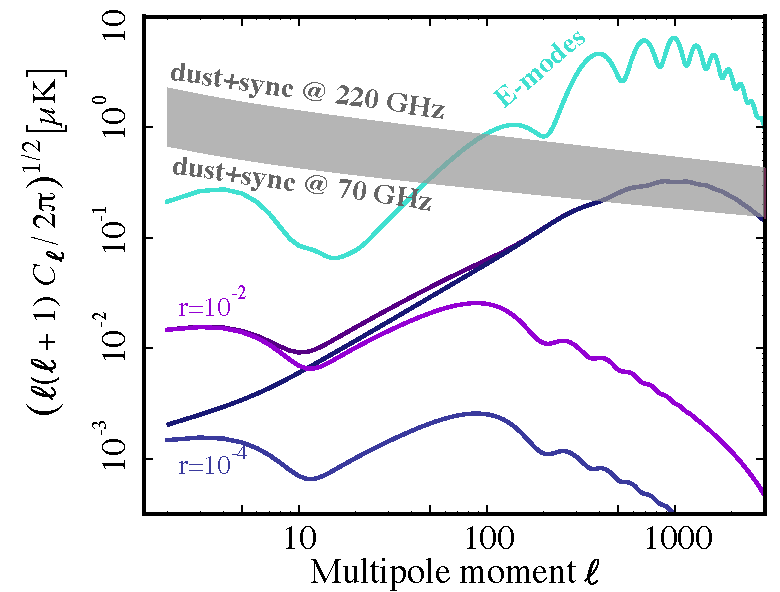
\includegraphics[width=2.9in]{Figures/cmb_vs_foreground.pdf}
\end{center}
\vspace{-0.25in}
\caption{\small \setlength{\baselineskip}{0.95\baselineskip}
{\it Left:} Brightness temperature as function of frequency for the polarized CMB (cyan, purple, blue)
and Galactic foreground signals: dust (red) and synchrotron (green). The darker bands correspond to
sky fractions between $73\%$ and $93\%$; the lighter bands to the cleanest $13\%$, with the width 
indicating the uncertainty. {\it Right:} Angular power spectra for inflationary, and for the sum 
of inflationary and lensing $B$ modes for two values of $r$; for $E$-mode polarization; 
and for foreground emission between 70 and 220~GHz.}
%, which shows the power spectrum of
%foregrounds over $75\%$ of the sky for frequencies between $70$ and
%$200$ GHz together with the lensing and inflationary contribution for
%different values of the tensor-to-scalar ratio.
\label{fig:frequency}
\vspace{-0.1in}
\end{figure}

\vspace{-0.18in}

\subsubsection{Foregrounds}
\label{sec:foregrounds}

\vspace{-0.05in}

Whereas the CMB temperature anisotropy signal dominates Galactic sources
of emission over much of the sky, this is not the case for polarization. 
Figure~\ref{fig:frequency} compares the expected RMS brightness temperature 
of polarized emission from Galactic sources to $E$ and $B$ modes
as a function of frequency and gives the expected signal levels as a function of angular scale $\ell$.  

\noindent The conclusions are that: \\
$\bullet$ \hspace{0.05in} over the largest angular scales (lowest $\ell$s), which are crucial for a range 
of science goals and where inflationary $B$ modes 
would be largest relative to those from lensing and instrument noise, foreground sources of confusion will need to be measured and subtracted to a level better than 1 part in 10 for $E$ and in 100 for $B$; \\
$\bullet$ \hspace{0.05in} foregrounds dominate the inflationary $B$ mode signal on {\it all} angular 
scales by an order of magnitude or more.

Known signals can be accounted for and removed even if their amplitude is large. 
But the best measurements to date, from \planck , have uncertainties that 
fall far short of the goals envisioned for the Probe. 
This is visually demonstrated by Figure~\ref{fig:Qrp001}, which 
compares the level of $B$ modes at low $\ell$ for $r = 0.001$ to the \planck\ 353 GHz noise, 
extrapolated to 150~GHz, a frequency band in which the inflationary signal is among the strongest. 
\begin{figure}[ht!]
\hspace{.05in}
\parbox{2.in}{\centerline {
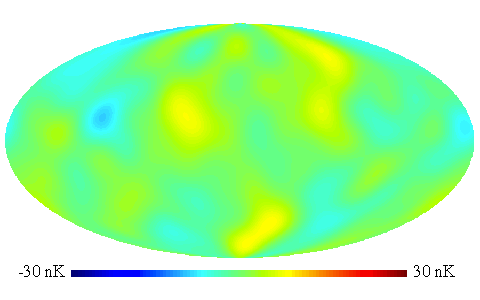
\includegraphics[width=2.1in]{Figures/P15_2_12_rp001.pdf} } }
%\hspace{-.05in}
\parbox{2.1in}{\centerline { 
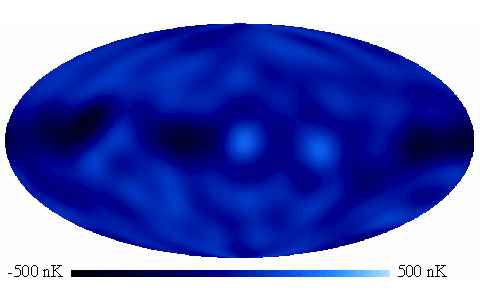
\includegraphics[width=2.1in]{Figures/P353_N_2_12.pdf} } }
\hspace{0.in}
\parbox{2.2in} { 
\caption{ \footnotesize \setlength{\baselineskip}{0.95\baselineskip}
{\it Left:} Stokes $Q$ for inflationary $B$ modes for $\ell<12$ and $r=0.001$. 
 {\it Right:} Noise in the $Planck$ 353~GHz map of Stokes $Q$ for $\ell<12$ 
 extrapolated to 150\,GHz assuming the (sky average) spectral properties of dust. 
 Note the color scales.  
\label{fig:Qrp001}  }  }
\vspace{-0.05in}
\end{figure}

%The extrapolation assumes the properties of dust as measured by \planck\ {\it on average} across
%the sky. We now know that these average properties are, as expected from fundamental physics, 
%only approximate. 
%\comred{say something about correlations, spatial distribution, variations in the spectral index. }

Removal of foregrounds based on multi-frequency data relies on extrapolations 
between frequencies based on an assumed spectral dependence. At the current level of precision a power law 
dependence for synchrotron radiation and a spatially uniform modified black body spectrum for dust emission 
give a reasonable fit to the data. But the complex composition of Galactic dust -- for example, the grains' size distribution, 
the different materials, and different radiative envirnoments -- suggests that this simple phenomenological description 
would no longer be valid at higher precision levels. One expects departures from a modified black 
body spectrum, and the emission properties are expected to vary spatially. 
The details of foreground emission, at every point on the sky, must 
ultimately be measured with the Probe itself. The challenge is to design the frequency 
coverage to do so optimally.  
%At the level of precision required for a probe mission, this description will no longer be 
%sufficient. The complex composition of dust leads to departures from a simple modified black body spectrum 
%because different components may emit at different temperatures. The different components are in general 
%not perfectly correlated with each other, leading to decorrelation between frequency bands. Furthermore, the 
%spectral dependence of synchrotron and dust emission is spatially varying. 

For $r<0.01$ the inflationary signal is at or below the lensing $B$ mode; see Figure~\ref{fig:clall}. 
Using high resolution polarization measurements, it is possible to reconstruct the lensing field and 
`delens' and thus remove the effect of lensing. But for low $r$ values significant delensing is 
required, and it is an open question at which point foregrounds will become the limiting factor. 

Good control of foregrounds is also necessary for the other science objectives. Detailed information 
about the reionization history, available by a cosmic variance limited measurement of the $E$ power spectrum, 
is buried below the foregrounds at $\ell < 10$. And 
recovering the spectral distortions signals will require proper accounting  of 
emission by dust grains, synchrotron emission from electrons spiraling in the Galactic magnetic 
field, Coulomb scattering of charged particles (`free-free', see Figure~\ref{fig:distortions}), 
as well as anomalous microwave and CO emission.   


%will be buried below the A satellite mission is likely also the only reliable way to measure the optical depth at a level necessary to break the degeneracy with the neutrino mass. 

%Nor is it clear that any set of sub-orbital measurements would provide a path for measuring 
%the foregrounds to the fidelity anticipated because the atmosphere limits the frequency 
%bands accessible, and because sub-orbital measurements are less stable and more prone
%to systematic uncertainties.  

% A mission aiming to detect primordial $B$ modes at this level across the sky will therefore not be able to rely on existing data. High signal-to-noise foreground measurements must accompany those at frequencies where the CMB contribution is larger.  As discussed below, optimizing the frequency coverage of these measurements will be a key goal of the mission concept study.

%Foregrounds 
%effect on reconstruction, and therefore subtraction of the lensing signal is not yet known.  will need to be measured 
%and controlled to 1 part if few tens, 

% \emph{Even in the cleanest patches of the sky}, polarized foreground emission is brighter than the sought-after primordial $B$ mode signal by over an order of magnitude at all frequencies.  This statement holds at all angular scales relevant to the search for primordial $B$ modes, as shown in the right panel of Figure~\ref{fig:frequency}.

%%%%%%%%% older text %%%%%%%%%

%A satellite mission provides a unique opportunity to target both the inflationary $B$-mode polarization that originates from the epoch of recombination and peaks around $\ell=80$ and the contribution that peaks on significantly larger scales $\ell\lesssim 12$. To measure the contribution from reionization will require an unprecedented understanding of foregrounds and systematic effects. This is illustrated in the left panel of Figure~\ref{fig:Qrp001}, which shows the contribution from reionization to the Stokes $Q$-parameter for $r=0.001$. The amplitude of the signal is approximately $10$ nK

%A satellite experiment enables
%full-sky observations, and provides 

%The CMB Probe has complete flexibility in the choice of frequency coverage, both of which are challenging from the ground or from the balloon platform.  Among other limitations, the atmosphere prevents observations at key frequencies, such as 60\,GHz, and requires data filtering that makes it difficult to recover the larger angular scales.

%By the time a probe-class mission launches, substantial progress will have been made in this quest.  In the absence of a primordial $B$ mode signal at detectable levels, the mission will significantly improve the upper limit on the tensor-to-scalar ratio $r$, with $\sigma(r)\!\sim\!10^{-3}$.  However, if $r$ is large enough, tentative $B$ mode detections could be reported from the ground or by ballon experiments ahead of this mission. The significance of such a discovery would be such that the detailed characterization of the angular and spectral dependence of the signal, as well as the verification of its isotropy across the sky, both of which are uniquely enabled by a satellite mission, would be required to confirm its primordial origin \comred{(cite Decadal Survey)}.

%In this scenario, a probe-class mission will in particular detect and characterize the reionization signal expected at the largest angular scales (multipoles below $\sim\!10$), where observations from other platforms are the most challenging. The contribution from reionization to the Stokes parameter $Q$ for $r=0.001$ is shown in the left panel of Figure~\ref{fig:Qrp001}. The amplitude of this signal is $\sim\!10$\,nK, which requires that any experiment attempting to measure it control large-scale foregrounds and systematics at the unprecedented level of a few nK.


%references
%Bruce+Fraisse2009 - 2009ApJ...696....1D
%Planck2015-IX - 2016A&A...594A...9P
%Planck2015-X - 2016A&A...594A..10P
%Planck2015-XXIX - A&A 586, A132 (2016)
%Planck2015-L - arXiv:1606.07335v1;
%Boulanger2016 - A&A 580, A136 (2015)
%Jewell2016 -  ApJ., 820, 2016
%





% Raphael, Josquin, Aurelien, Charles, Graca
